\section{Theory}

	The Analog to Digital Converter (ADC) converts analog signals to digital signals while the Digital to Analog Converter (DAC) converts digital signals to analog signals. In this experiment, we will construct and study the working of an ADC and a DAC using dedicated Integrated Circuits (ICs) instead of using basic electronic components. This circuit diagram is shown in \hyperref[th:1]{\textbf{Figure 1}}.

	\begin{figure}[H]
		\centering
		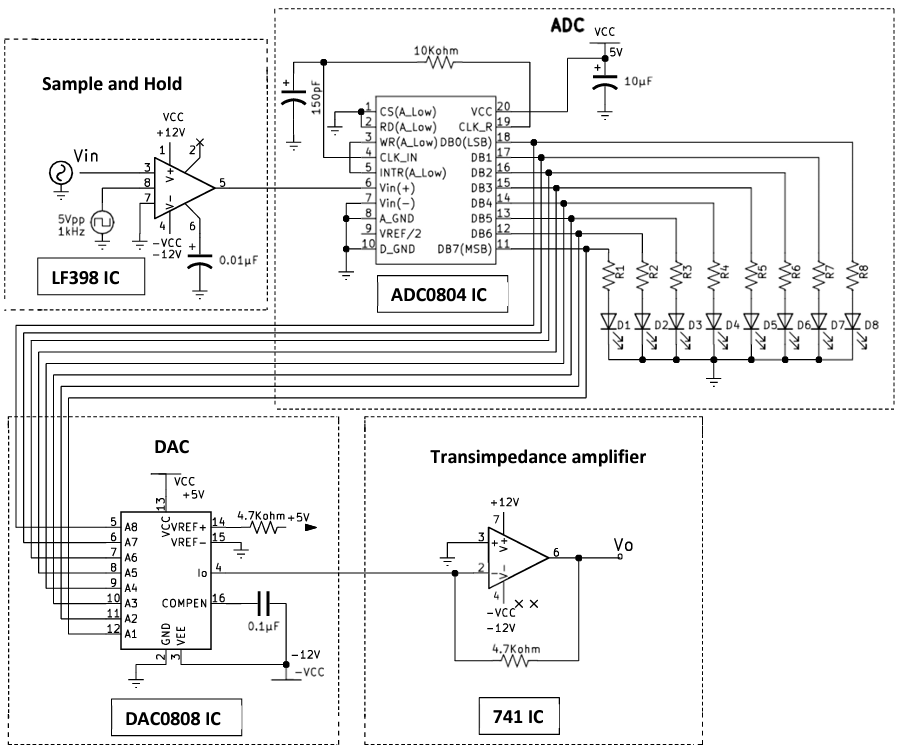
\includegraphics[width=\columnwidth]{images/theory1.png}
		\caption{Circuit for ADC-DAC with sample and Hold}
		\label{th:1}
	\end{figure}

	Compared to the previous circuit, this circuit is much simpler and does not require a priority encoder, while also working with a larger number of bits. The circuit diagram for the experiment is shown below.

		\begin{figure}[H]
			\centering
			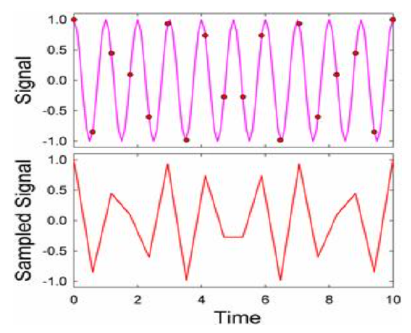
\includegraphics[width=0.6\columnwidth]{images/theory3.png}
			\caption{Aliased Sampled output for sampling rate violating Nyquist theorem}
			\label{th:2}
		\end{figure}

	\subsection{Nyquist Frequency}

		The Nyquist frequency is the minimum sampling rate required for accurate representation of an analog signal in digital form. If the signal is sampled at a rate below the Nyquist frequency, the resulting digital signal will not accurately represent the original analog signal. The Nyquist frequency is defined as half the sampling rate.

		\begin{figure}[H]
			\centering
			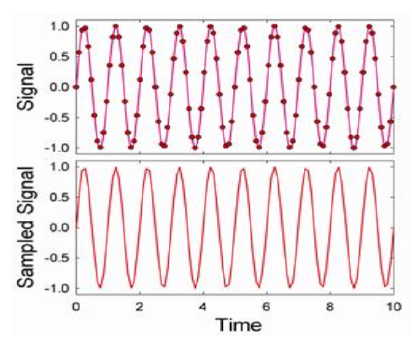
\includegraphics[width=0.6\columnwidth]{images/theory2.png}
			\caption{Sampled output that is a good approximation of the input signal}
			\label{th:3}
		\end{figure}
		
		As shown in \hyperref[th:2]{\textbf{Figure 2}}, violating Nyquist's theorem can result in aliasing, which is when signals at higher frequencies get shifted down to lower frequencies. On the other hand, \hyperref[th:3]{\textbf{Figure 3}} demonstrates a good approximation of the input signal using a properly sampled output.

	\subsection{Sample and Hold Circuit}

		The sample and hold circuit is shown in Figure 1 and is constructed with the LF398 IC. The purpose of this circuit is to sample the input signal and hold it until it is converted to digital format. The sample and hold circuit discretizes a continuous input AC signal by capturing the signal at an instant of time and holding it via hold mode (using capacitors).

		It requires an external clock signal for its operation which is supplied using a function generator. Approximation accuracy depends on the sampling rate and resolution. The sampling frequency ($f_z$) should be more than twice the maximum frequency present in the signal, also known as the Nyquist frequency. If we violate Nyquist's theorem we get aliasing; signals at higher frequencies get shifted down to lower frequencies as shown in Figure 2.

		The output digital signal from the sample and hold circuit is fed to an 8-bit ADC IC, which then outputs a digital signal. This digital signal is then fed to an 8-bit DAC IC for digital to analog conversion. Sampling and holding is important for proper conversion of analog signals, which we encounter every day in the lab. All multichannel analyzers also use ADC.

	\subsection{Analog to Digital Converter (ADC)}

		The ADC circuit is constructed with an ADC0804 IC, which is an 8-bit successive approximation ADC converter. The circuit involves a sample and hold component for sampling the input AC signal and feeding it to the ADC IC. The sample and hold circuit is constructed using an LF398 IC, which discretizes a continuous input AC signal by capturing the signal at an instant of time and holding it via hold mode (using capacitors). The ADC IC also utilizes an internal clock to give clock pulse to the sample and hold circuit, but it is not used in this experiment due to noise in the clock pulse signal.

	\subsection{Digital to Analog Converter (DAC)}

		The DAC circuit is constructed using a DAC0808 IC, which is an 8-bit DAC chip with an R-2R ladder. For this experiment, we are using a dual in-line package. The output of this IC is given by the equation:
		
		\begin{equation}
			I_0 = K \left(\frac{A_1}{2^1} + \frac{A_2}{2^2} + \frac{A_3}{2^3} + \frac{A_4}{2^4} + \dots \right)
			\label{eq:1}
		\end{equation}

		where $K = \frac{V_{Ref}}{R}$, $K_{ref} = 5V$, and $R = 4.7k\Omega$.
	
	\subsection{Transimpedance Amplifier}

		A transimpedance amplifier is an electronic circuit that converts current to voltage. It is a current-to-voltage converter that is constructed using an operational amplifier such as the 741 IC. Compared to other methods of current-to-voltage conversion, the transimpedance amplifier has superior impedance characteristics due to its low input impedance and high output impedance. This results in a higher gain, making it a much better method of current-to-voltage conversion than using an ordinary resistor. The transimpedance amplifier is commonly used in a variety of applications, such as in photodiodes, where it converts the current generated by the diode to a voltage signal.